%%%%%%%%%%%%%%%%%%%%%%%%%%%%%%%%%%%%%%%%%%%%%%%%%%%%%%%%%%%%%%%%%%%%%%%%%%%%%%%%
\chapter{Анализ подходов к автоматической модификации программного кода}
%%%%%%%%%%%%%%%%%%%%%%%%%%%%%%%%%%%%%%%%%%%%%%%%%%%%%%%%%%%%%%%%%%%%%%%%%%%%%%%%

Ссылка на статью\cite{javascript}

Ссылка на сайт\cite{ANTLR}

Ссылка на книгу\cite{java-book}

\section{Automatically Fixing Real-World JavaScript Performance Bugs}

\nomenclature{АСД}{Абстрактное синтаксическое дерево, AST}

\section{IntelliJ IDEA Quick Fix}

Ссылка на рисунок \ref{fig:idea}.

\begin{figure}[htbp]
	\centering
	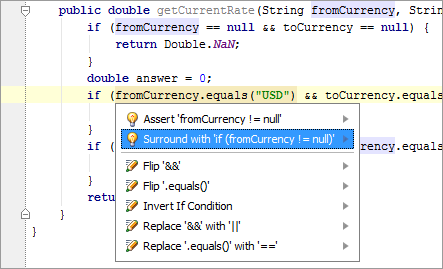
\includegraphics[width=0.8\textwidth]{fig/code_analysis_bugs.png}
	\caption{Предупреждение от статического анализатора в IntelliJ IDEA и всплывающее меню Quick Fix}%
	\label{fig:idea}
\end{figure}